\documentclass[12pt]{article}

\usepackage[margin=1in]{geometry}

\usepackage{amsmath, graphicx, caption, subcaption, xcolor}

% Today I learned about resizing brackets and parentheses \left and \right

\graphicspath{{res/}}

\title{Gathering Sun Fringe Frequencies with an Interferometer}
\author{Lukas Finkbeiner}

\begin{document}

\maketitle

\begin{abstract}

We initially set out with the great ambition to explore interferometery and its application toward the mapping and measurement of the Sun, the Moon, and Cygnus A. However, due to dramatic failures in our data-taking, the scope of this report is limited to an incomplete discussion of fringe frequencies for the Sun. We find our data for the Sun agrees with our model, with a worst percent error of approximately ten. We dedicate the remainder of the paper to a discussion of erroneous data as well as, briefly, the capacity to which some of them could be salvaged.

\end{abstract}

\section{Introduction and Background}

\begin{equation}
F(h_s) = A \cos (2 \pi \nu \tau_g') + B \sin (2 \pi \nu \tau_g')
\end{equation}

This is the equation we use to calculate expected fringe amplitudes F of a point source as a function of the hour angle $h_s$ of a point source in terms of $A \equiv \cos(2 \pi \nu \tau_c')$ and $B \equiv -\sin(2 \pi \nu \tau_c')$. In this paper, we make larger use of a related concept, fringe frequency:

% I cannot follow how one would transform back from the resuts. We run into plenty of other terms like B_{ew} and B_{ns} which I don't think we know. Maybe L, \delta, and h_s do not depend on time, so this $could$ make sense...

\begin{equation} \label{eq:lff}
f_f = \left[ \frac{B_{ew}}{\lambda} \cos \delta \right] \cos h_{s, 0} - \left[\frac{B_{ns}}{\lambda} \sin L \cos \delta\right] \sin h_{s, 0}
\end{equation}

%The hour-angle and declination of the Sun and Moon change as they traverse the sky.

Measuring the Diameter of a Circular Source $[\frac{B_{ew}}{\lambda} \cos \delta]$

\begin{equation}
I(\Delta h) = \frac{(R^2 - \Delta h^2)^{1/2}}{R}
\end{equation}

\begin{equation}
\begin{split}
MF_\text{theory} &= \frac{1}{R} \int_{-R}^R \left( R^2 - \Delta h^2 \right)^{1/2} \cos \left( 2 \pi f_f \Delta h \right) d \Delta h \\
&\approx \frac{1}{R} \sum_{n = -N}^{n = +N} \left[ R^2 - (n\delta h)^2 \right]^{1/2} \cos \left( 2 \pi f_f n \delta h \right) \delta h \\
&= \delta h \sum_{n = -N}^{n = +N} \left[ 1 - \left( \frac{n}{N} \right)^2 \right]^{1/2} \cos \left(\frac{2 \pi f_f R n}{N} \right)
\end{split}
\end{equation}

where $B_{ew} \approx 20$ m, $B_{ns} \sim 0$ m, $\lambda \approx 2.5$ cm.

We have one null (figure \ref{fig:Sun_null}) from our Sun hour-long capture. We cannot perform extensive analysis with such a short window of time. For example, consider a radius calculation, which depends on the number of nulls in our data: our one parameter would absorb all of the error.

\section{Methods}

\quad \quad To observe the Sun, Moon, and Cygnus A, we used an East-West ($B_{ns} ~ 0$ m) interferometer with two antennae.

We used the ugradio interface with the antennae. To accomplish our goals, we implemented additional features in a dedicated data-taking script. Our first iteration involved a user-specified target function; this function would compute the current altitude and azimuth of the target so that the script could point the dish, record data for about one minute, then point again.

Our data-taking script passed through multiple iterations over the course of the overarching project. Most of these changes patched minor crashes and slight errors in pointing. More importantly, we added several levels of record-keeping. Initially, we simply took (voltage, time) tuples from the ugradio multimeter interface and manually re-calculated where the dish should have been pointing at given the time as well as the target (i.e. Moon, Sun, Cygnus A). The script was at this stage when we recorded the hour of Sun data that we use here.

Then, after concerns about the veracity of our pointing commands, we began to record the altitudes and azimuths that the script had automatically computed; we had hoped to identify a pointing mistake by comparing the automatically computed angles with our manually computed angles for the same time range. The script was at this stage when we performed the horizon-to-horizon captures of the Moon and Cygnus A that we use here.

\begin{figure}
	\centering
	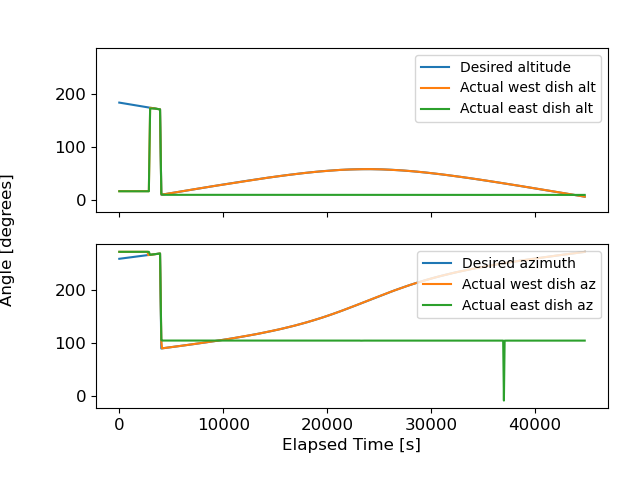
\includegraphics[width=.6\linewidth]{lockup}
	\caption{These are the comparisons between the input dish angles (as computed with rotation matrices) and the true angles as reported by the dishes. The east dish displays little to no response, indicating that it was stuck for the virtually the entire capture.}
	\label{fig:stuck}
\end{figure}

Finally, we further expanded the book-keeping array to include the $actual$ altitudes and azimuths of the two antennae as reported by the antennae. This was a late addition to the script, so we only have this level of information for our Sun horizon-to-horizon capture (figure \ref{fig:stuck}). However, as we discuss in the appendix, this could likely have been the most important addition.

\section{Observations}

\quad \quad The vast majority of the data appeared to be unusable. We are only able to strongly justify this claim for the last full Sun set, but some evidence for the previous collections is discussed in the appendix. This is also where a selection of the unused data appear, in the form of plots.

\begin{figure}
	\centering
	\includegraphics[width=.6\linewidth]{envelope/Sun_hour}
	\caption{Raw data from our hour-long Sun observation on 3/12. Excepting a control conflict (which resulted in the dip near 1500 seconds), the data largely match expectation. Although we lack a form of confirmation analogous to figure \ref{fig:stuck}, the strength of the match of the data to the expectation indicates that the dishes successfully responded to our pointing commands.}
	\label{fig:Sun_envelope}
\end{figure}

\begin{figure}
	\centering
	\includegraphics[width=.6\linewidth]{sinusoid/Sun_hour}
	\caption{We zoom in on an arbitrary segment of figure \ref{fig:Sun_envelope} to show the presence of a smooth local sinusoid within the envelope.}
	\label{fig:Sun_sinusoid}
\end{figure}

\begin{figure}
	\centering
	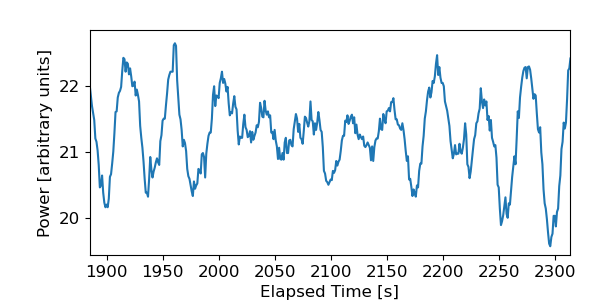
\includegraphics[width=.6\linewidth]{null}
	\caption{We zoom in on the segment of figure \ref{fig:Sun_envelope} corresponding to the envelope's region of lowest amplitudes. Near the null ($\approx$ 2100 s) of the signal, we see a reflection without inversion.}
	\label{fig:Sun_null}
\end{figure}

\section{Analysis}

\quad \quad Consider our local fringe frequency equation \ref{eq:lff}. We plug in for known values and convert to cycles per second:

\begin{equation} \label{eq:fringes_expect}
f_f = \left[ 800 \cos \delta \right] \cos h_{s, 0} \times \frac{2 \pi}{60 \times 60 \times 24} \approx \frac{\cos \delta \cos h_{s, 0}}{17.19}
\end{equation} 

The recording of the Sun ran from 9:03:19 am to 10:07:02 am on Thursday 3/12. We define the meridian to be $h_s = 0$, and a full solar day to be $2\pi$ radians. Then, we find that the hour angle ranges, approximately, from $-0.7709$ to $-0.4888$. This allows us to construct a plot of, as a function of time, the expected and observed fringe frequencies of the Sun (figure \ref{fig:Sun_fringes}). We see that the percent error is as large as ten percent with the first observation, but that the model and observations seem to agree at greater values of time. Alternatively, one can see there is perhaps a dip in discrepancies around the center, which suggests that the null contributes to the narrowing of error.

\begin{figure}
	\centering
	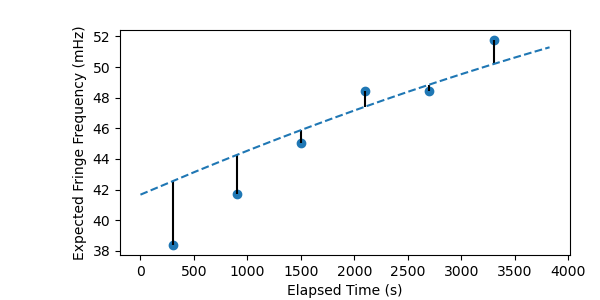
\includegraphics[width=.6\linewidth]{yeah_thatsright}
	\caption{A plot of the fringe frequencies calculated by ten-minute windows in the Sun data. The dashed line represents the values we would expect, based on equation \ref{eq:fringes_expect}.}
	\label{fig:Sun_fringes}
\end{figure}

We largely disregard our results for the Moon and Cygnus A, but we add, as an interesting note, our plots for observed fringe frequencies. They potentially speak about the effectiveness of a single interferometer. However, I could not guess as to how a single interferometer could recover useful data if the interferometer by construction multiplies the two antannae's signals together, and one antenna points to what we can mathematically approximate as, on average, a random patch of the sky. 

Figure \ref{fig:Moon_fringes} shows a patchy trend of the fringe frequency moving up and then down over the course of the whole capture. This would agree with our model. Figure \ref{fig:CygA_fringes} is less consistent. We would expect that the fringe frequency of a point source does not change much as it traverses the sky, so it is at least reassuring that the plot lacks a clear pattern (perhaps representing noise around a point). These plots were independently verified at several places, to make sure that the fringe calculator was operating appropriately.

\begin{figure}
	\centering
	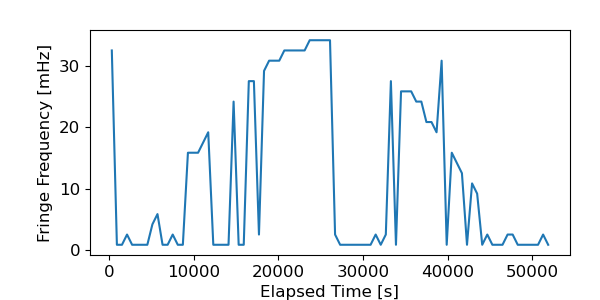
\includegraphics[width=.6\linewidth]{fringes/Moon_fringe}
	\caption{A plot of the fringe frequencies calculated by ten-minute windows in the Moon data. We see that only the largest dip (near 30000 seconds) corresponds to the raw data (figure \ref{fig:Moon_envelope}). Consequently, only so much information can be salvaged.}
	\label{fig:Moon_fringes}
\end{figure}

\begin{figure}
	\centering
	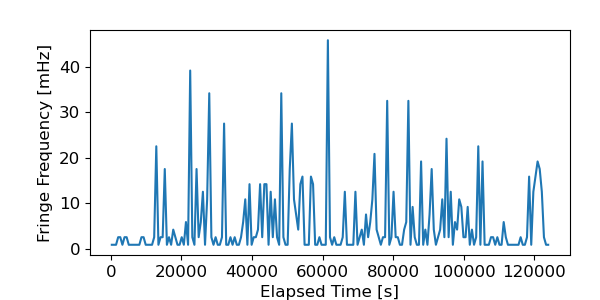
\includegraphics[width=.6\linewidth]{fringes/Cyg_fringe}
	\caption{A plot of the fringe frequencies calculated by ten-minute windows of the Cygnus A data. We see a sporadic pattern of spikes of varying magnitudes; it is less clear that there is a salvageable picture from these data.}
	\label{fig:CygA_fringes}
\end{figure}

\section{Conclusions}

\quad \quad Perhaps the single greatest obstacle to our data collection turned out to be the freezing of the antennae (which our group found not to resolve itself even over a horizon-to-horizon capture). Initially, we had written the script to automatically raise an exception whenever there was a discrepancy of greater than one fifth of a degree between the just-repositioned antennae's self-reported angles and the angles that we had requested. For reasons still unknown, the script kept raising exceptions even when my parallel inquiries showed that the antennae did in fact agree. In any case, we failed to procure, on time, a script that would automatically detect antennae freezing.
 
Therefore, the situation called for the manual spotting of antenna failures. However, this raises its own set of issues. Even with the latest version of our data-taking script, the failure of a dish can take a while to show up in the data. Consider the magnitudes along the x-axis of figure \ref{fig:stuck}. Consider, especially, how the gap closed between the azimuths of the two antennae from about 5000 to 10000 seconds. That is a span of about an hour over which it was not clear to me whether the problem would resolve itself. Furthermore, even after deciding that the dishes must be stuck, there was a miscommunication over Piazza and the dishes were not corrected in time for this measurement.
 
Even without miscommunication, the mere human-mediated nature of requesting a reset of antennae inevitably leads to large delays. Still, one would potentially obtain enough data in order to perform   a basic set of analyses. To re-iterate, the optimal approach to this project would have been to fix the script angle-discrepancy detection. Then, in the worst case, we would have lost about an hour of data for each run. Here, we seem to have lost everything, except, potentially out of luck, for the one Sun hour.

\section{Acknowledgments}

\quad \quad Mehdi wrote most of the original code used for capturing and recording data from the interferometer. Rebecca and I collected the data and tweaked the scripts along the way.

Theory and background provided by Aaron Parsons. ``LAB 3: Radio Interferometery at X-Band.'' Updated March 2020.

\section{Appendix: on Poor Data}

\quad \quad This last portion of the report contains the data which we deemed unusable for the report.

We may observe what appears to be a $local$ sinusoid in the Moon (figure \ref{fig:Moon_sinusoid}) and Cygnus A point-source (\ref{fig:Cyg_sinusoid}) data, but the notion of an envelope does not agree strongly with the erratic jumps and long meandering trend-lines of the big-picture views (figures \ref{fig:Moon_envelope} and \ref{fig:Cyg_envelope}).

\begin{figure}
	\centering
	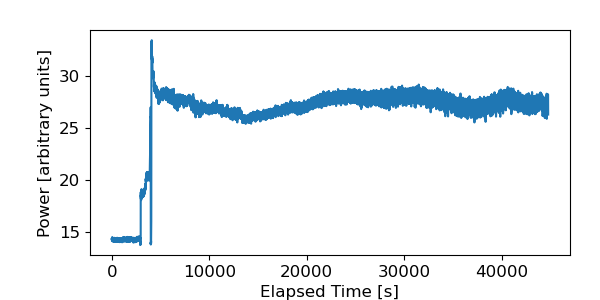
\includegraphics[width=.6\linewidth]{envelope/Sun_h2h}
	\caption{An overview of the Sun data for the horizon-to-horizon capture (Friday, April 3). Technically, $these$ are the only data which figure \ref{fig:stuck} directly explains. However, figures \ref{fig:Moon_envelope} and \ref{fig:Cyg_envelope} also lack a familiar envelope.}
	\label{fig:Sun_h2h_envelope}
\end{figure}

\begin{figure}
	\centering
	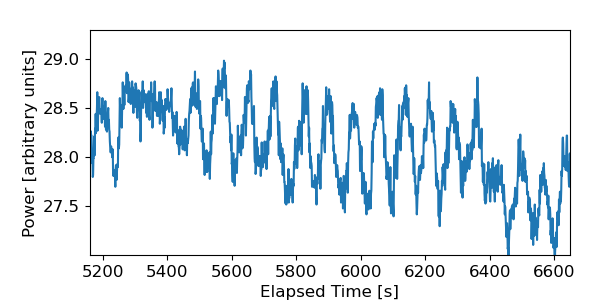
\includegraphics[width=.6\linewidth]{sinusoid/Sun_h2h}
	\caption{We zoom in on a segment of figure \ref{fig:Sun_h2h_envelope} to show that, despite one dish freezing, we could be misled by a local sinusoid. We were able to recover a similarly-jagged local sinusoid from our Moon horizon-to-horizon capture (figure \ref{fig:Moon_sinusoid}). Therefore, our Moon data are consistent with this model of a dish failure.}
	\label{fig:Sun_h2h_sinusoid}
\end{figure}

\begin{figure}
	\centering
	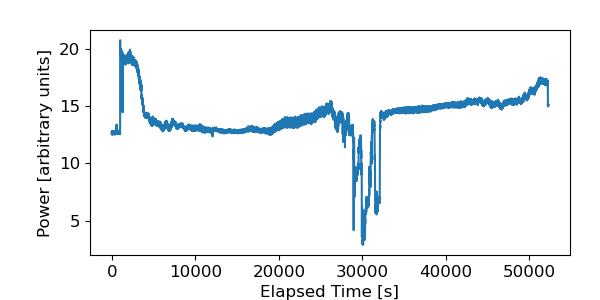
\includegraphics[width=.6\linewidth]{envelope/Moon}
	\caption{This is an overview of our `Moon' data (most likely, one dish pointed at the Moon while the other maintained constant azimuth and altitude). One might argue that the major jumps in the plot could be explained by script failures or the Moon passing behind some solid surface. In any case, there does not appear to be an envelope (corresponding to a well-known function, at least) over any section of these data.}
	\label{fig:Moon_envelope}
\end{figure}

\begin{figure}
	\centering
	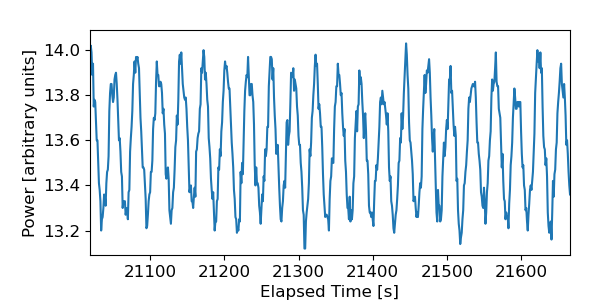
\includegraphics[width=.6\linewidth]{sinusoid/Moon}
	\caption{When we zoom in on a typical section, in this case roughly nine minutes, we can see a periodic pattern in the received power. The shape of the cycle indicates a local sinusoid.}
	\label{fig:Moon_sinusoid}
\end{figure}

\begin{figure}
	\centering
	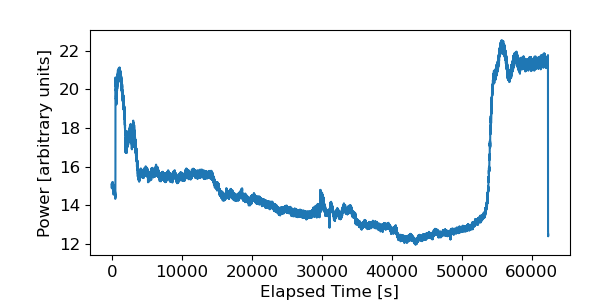
\includegraphics[width=.6\linewidth]{envelope/CygnusA}
	\caption{This is an overview of our `Cygnus A' data (likely that one dish pointed at Cygnus A while the other maintained constant azimuth and altitude). As in figure \ref{fig:Moon_envelope}, there does not appear to be a consistent envelope over any section of these data.}
	\label{fig:Cyg_envelope}
\end{figure}

\begin{figure}
	\centering
	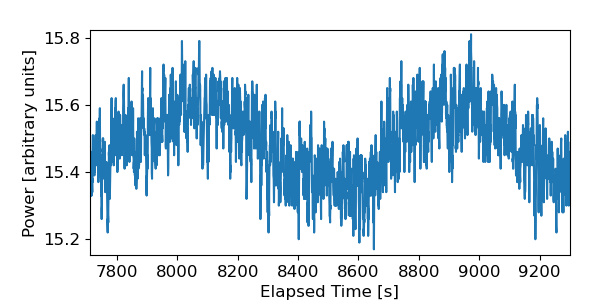
\includegraphics[width=.6\linewidth]{sinusoid/CygnusA}
	\caption{We zoom in on the Cygnus A data to show some of the large-period sinusoids that crop up in most places. To be sure, the periods of these sinusoids are much larger than those of the Moon's (figure \ref{fig:Moon_sinusoid}), so this is potentially not a $local$ sinusoid at all, but rather some coincidental envelope artifact.}
	\label{fig:Cyg_sinusoid}
\end{figure}

\end{document}
